% chapters/04_bridges.tex — Publication grade (standardized, narrow-safe)
\chapter{Bridges: Thermodynamics \& Information \\ \large RCFT — working theory}
\label{ch:bridges}

\begin{callout}[RCFT — scope]
This chapter offers \emph{analogies} that help interpret the First-Law budget (Chapter~\ref{ch:firstlaw}) through lenses from thermodynamics and information theory. These are \textbf{closures}, not identities. Every claim here is paired with limits and falsifiers. The kernel remains the canonical budget
\[
\Delta\kappa \stackrel{!}{=} R\,\tau_{R} - \bigl(D_{\omega}+D_{C}\bigr),
\]
and the integrity proxy
\[
\mathrm{IC} = F\,e^{-S}\,(1-\omega)\,\exp\!\left(-\alpha\,\frac{C}{1+\tau_{R}}\right),
\qquad \kappa=\ln(\mathrm{IC}).
\]
\end{callout}

\section{Budget mappings (thermodynamics \& information)}
We map budget terms to \emph{work/heat}-like and \emph{code-length} viewpoints. Treat the mapping as a mnemonic; limits are stated below.

\begin{eqbox}[Mnemonic mappings (RCFT)]
\small
\begin{tabularx}{\linewidth}{@{}>{\bfseries}l X@{}}
$R\,\tau_{R}$ & work-like organized return (useful ordering) \\
$D_{\omega}$  & heat-like drift dissipation (randomization) \\
$D_{C}$       & geometric/curvature cost (bending the landscape) \\
$S$           & code-length / surprisal proxy ($\approx -\ln(1-\omega+\varepsilon)$) \\
$F$           & channel fidelity (recoverable fraction) \\
$1-\omega$    & survival factor / compression headroom \\
\end{tabularx}
\end{eqbox}

\paragraph{Thermodynamic lens.}
Read $R\,\tau_{R}$ as “organized return” (work-like) and $D_{\omega}+D_{C}$ as “dissipative” charges (heat-like). Ordered return must pay for drift/curvature to yield net $\Delta\kappa$.

\paragraph{Information-theoretic lens.}
With
\[
\kappa \;=\; \ln F \;-\; S \;+\; \ln(1-\omega) \;-\; \alpha\,\frac{C}{1+\tau_{R}},
\]
$S$ acts like a \emph{code-length} penalty (surprisal), $\ln(1-\omega)$ a headroom/compressibility term, and the curvature fraction a structured penalty per unit geometry over the available return window $(1+\tau_R)$.

\subsection*{Limits of the analogy}
\begin{itemize}[leftmargin=1.8em]
  \item Not a thermodynamic state equation; no guaranteed Maxwell relations.
  \item $R$ is a return rate, not a mechanical force; $D_C$ is geometric, not thermal.
  \item The code-length picture assumes quasi-stationarity on the audited interval.
  \item Near $\omega\to1$, the guard $\varepsilon$ is numerical, not a physical entropy floor.
\end{itemize}

\section{Sensitivities (first-order response)}
From the proxy above, holding other terms fixed on a slice,
\[
\frac{\partial \kappa}{\partial C} = -\frac{\alpha}{1+\tau_{R}}, 
\qquad
\frac{\partial \kappa}{\partial \tau_{R}} = \frac{\alpha\,C}{(1+\tau_{R})^{2}}.
\]

\begin{eqbox}[Sensitivity card]
\[
\boxed{\;\Delta \kappa \;\approx\; 
\frac{\partial \kappa}{\partial C}\,\Delta C \;+\;
\frac{\partial \kappa}{\partial \tau_{R}}\,\Delta \tau_{R}\;}
\quad=\quad
-\frac{\alpha}{1+\tau_{R}}\,\Delta C \;+\; \alpha\,\frac{C}{(1+\tau_{R})^{2}}\,\Delta \tau_{R}.
\]
\textbf{Signs:} increasing $C$ reduces $\kappa$; decreasing $\tau_R$ increases $\kappa$, with diminishing returns as $\tau_R$ grows.
\end{eqbox}

\paragraph{Costs (local).}
A unit curvature injection ($\Delta C=+1$) drops $\kappa$ by $\alpha/(1+\tau_R)$. A unit return shortening ($\Delta\tau_R=+1$ in speed units) raises $\kappa$ by $\alpha\,C/(1+\tau_R)^2$.

\section{Falsifiers \& testable predictions}
Design small perturbations on a slice; compare measured $\Delta\kappa$ with the linear prediction. Use the Budget Report residual as the absolute tolerance.

\subsection*{Test 1 — Curvature injection}
\textbf{Setup.} Hold $\omega,\,F,\,S,\,\tau_R$ roughly fixed; increase $C$ by $\Delta C$.  
\textbf{Prediction.} $\Delta\kappa \approx -\dfrac{\alpha}{1+\tau_R}\,\Delta C$.  
\textbf{Example.} $\alpha=1$, $\tau_R=3.0$, $\Delta C=0.10 \Rightarrow \Delta\kappa \approx -0.033\bar{3}$.  
\textbf{Falsifier.} Sign flip or magnitude error beyond tolerance.

\subsection*{Test 2 — Return shortening}
\textbf{Setup.} Hold $\omega,\,F,\,S,\,C$ fixed; reduce $\tau_R$ by $\Delta\tau_R>0$.  
\textbf{Prediction.} $\Delta\kappa \approx \dfrac{\alpha\,C}{(1+\tau_R)^2}\,\Delta\tau_R$.  
\textbf{Example.} $\alpha=1$, $C=0.20$, $\tau_R=2.0$, $\Delta\tau_R=0.5 \Rightarrow \Delta\kappa \approx 0.0111$.  

\subsection*{Test 3 — Near-wall cubic fall}
\textbf{Setup.} Sweep $\omega$ upward with other terms steady.  
\textbf{Prediction.} $\mathrm{IC}\propto (1-\omega)^3$ (log–log slope $\approx3$ vs.\ $(1-\omega)$).  
\textbf{Falsifier.} Systematic slopes $\ll3$ away from guard bands.

\section{What \emph{not} to claim (guardrails)}
\begin{itemize}[leftmargin=1.8em]
  \item Do not equate $R$ with force or $D_{\omega}$ with temperature without a separate, audited identification.
  \item Do not read $S$ as thermodynamic entropy absent an admissible ensemble.
  \item Do not treat $\kappa$ as free energy; its units are those of \emph{log-integrity} with a conventional zero.
\end{itemize}

\section{Caption pattern for RCFT figures}
\begin{eqbox}[Caption checklist (RCFT one-liner)]
\small
\begin{tabularx}{\linewidth}{@{}>{\bfseries}l X@{}}
Pattern & \emph{Figure X.Y — Title (RCFT)}. Contract $(a,b,\varepsilon,p,\alpha)$; channels; prediction (formula); observed (numbers); residual $<10^{-12}$; limits (stationarity/near-wall); weld \texttt{<id>}; manifest \texttt{<sha256>}. \\
\end{tabularx}
\end{eqbox}

\section{Schematic figures (guarded includes)}

\begin{figure}[h]
  \centering
  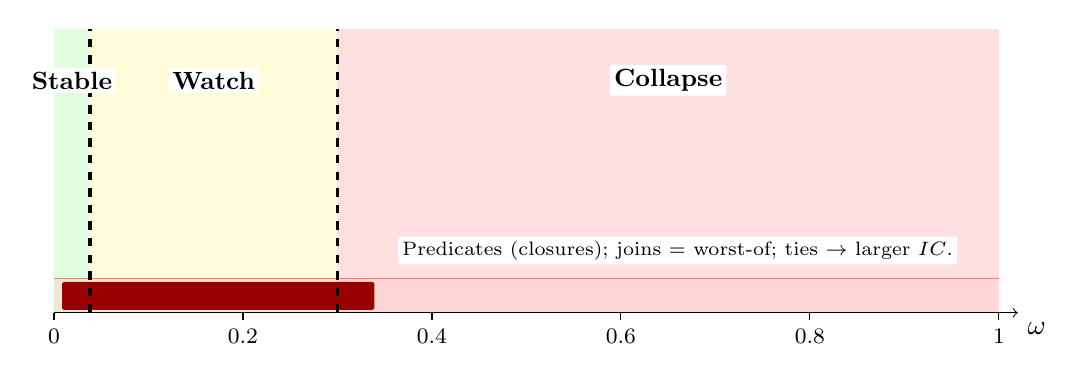
\begin{tikzpicture}[x=12cm,y=3.6cm]
    % --- styles ---
    \tikzset{labelbox/.style={fill=white,rounded corners=0.6pt,inner sep=1.5pt}}

    % background bands (regime gates by ω)
    \fill[green!12] (0,0) rectangle (0.038,1);
    \fill[yellow!15] (0.038,0) rectangle (0.30,1);
    \fill[red!12]    (0.30,0) rectangle (1,1);

    % Critical overlay ribbon (IC < 0.30) — translucent rectangle + label
    \fill[red!25,opacity=0.30] (0,0) rectangle (1,0.12);
    \draw[red!55] (0,0.12) -- (1,0.12);
    \node[labelbox,anchor=west,red!60!black] at (0.008,0.06)
      {\footnotesize \textbf{Critical overlay:} $IC<0.30$};

    % axis (ω) with tidy ticks
    \draw[->] (0,0) -- (1.02,0) node[below right] {$\omega$};
    \foreach \x/\lbl in {0/0,0.2/0.2,0.4/0.4,0.6/0.6,0.8/0.8,1/1}%
      \draw (\x,0) -- ++(0,-0.025) node[below,font=\footnotesize] {\lbl};

    % threshold lines
    \draw[dashed,very thick] (0.038,0) -- (0.038,1);
    \draw[dashed,very thick] (0.30,0) -- (0.30,1);

    % regime labels (top, centered in each band)
    \node[labelbox,font=\small\bfseries] at (0.019,0.82) {Stable};
    \node[labelbox,font=\small\bfseries] at (0.169,0.82) {Watch};
    \node[labelbox,font=\small\bfseries] at (0.65,0.82)  {Collapse};

    % compact join note (no overlap with ribbon)
    \node[align=left,font=\scriptsize,labelbox] at (0.66,0.22)
      {Predicates (closures); joins = worst-of; ties $\rightarrow$ larger $IC$.};
  \end{tikzpicture}

  \caption{Regime thresholds and joins (defaults) with Critical overlay. Vertical markers at $\omega=0.038$ and $\omega=0.30$ indicate the Stable/Watch/Collapse cuts. The translucent ribbon marks the \emph{Critical overlay} ($IC<0.30$) which can occur anywhere in $\omega$. 
  Inequalities: Stable ($\omega<0.038$), Watch ($0.038\le\omega\le0.30$), Collapse ($\omega>0.30$). 
  \textbf{Contract}: $(a,b,\varepsilon,p,\alpha)=(-3.7280384,\,10.856631,\,10^{-8},\,3,\,1.0)$. 
  \textbf{Face policy}: \texttt{post\_clip+guard}. 
  \textbf{Budget}: not applicable (schematic).}
  \label{fig:regime-thresholds}
\end{figure}


\begin{figure}[h]
  \centering
  % Plain TikZ; no extra libraries required
  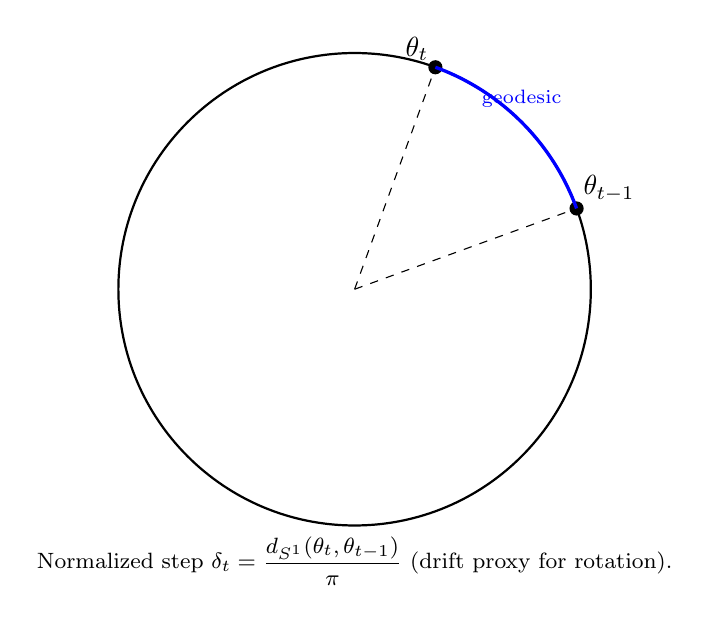
\begin{tikzpicture}[scale=3.0]
    % unit circle
    \draw[thick] (0,0) circle (1);
    % choose two angles (degrees)
    \def\thA{20}   % theta_{t-1}
    \def\thB{70}   % theta_t
    % points
    \coordinate (O) at (0,0);
    \coordinate (A) at ({cos(\thA)},{sin(\thA)});
    \coordinate (B) at ({cos(\thB)},{sin(\thB)});
    % radii
    \draw[dashed] (O) -- (A);
    \draw[dashed] (O) -- (B);
    % points
    \fill (A) circle (0.03);
    \fill (B) circle (0.03);
    \node[above right=-1pt] at (A) {$\theta_{t-1}$};
    \node[above left=-1pt]  at (B) {$\theta_{t}$};
    % geodesic (shortest arc) — plain thick arc, no decorations
    \draw[very thick,blue] (A) arc[start angle=\thA, end angle=\thB, radius=1];
    % label near midpoint of arc
    \node[blue] at ({cos((\thA+\thB)/2)},{sin((\thA+\thB)/2)+0.10}) {\scriptsize geodesic};
    % explanatory label
    \node at (0,-1.15) {\footnotesize Normalized step $\displaystyle \delta_t=\frac{d_{S^1}(\theta_t,\theta_{t-1})}{\pi}$ (drift proxy for rotation).};
  \end{tikzpicture}

  \caption{Geodesic step on $S^1$: two angles $\theta_{t-1}$, $\theta_t$ on the unit circle with shortest arc (geodesic) shown; normalized step $\delta_t=d_{S^1}(\theta_t,\theta_{t-1})/\pi$ serves as a drift proxy for rotation channels.
  \textbf{Contract}: $(a,b,\varepsilon,p,\alpha)=(-3.7280384,\,10.856631,\,10^{-8},\,3,\,1.0)$.
  \textbf{Budget}: not applicable (schematic).}
  \label{fig:rotation-geodesic-s1}
\end{figure}

\begin{figure}[h]
  \centering
  % Plain TikZ axes; no pgfplots
  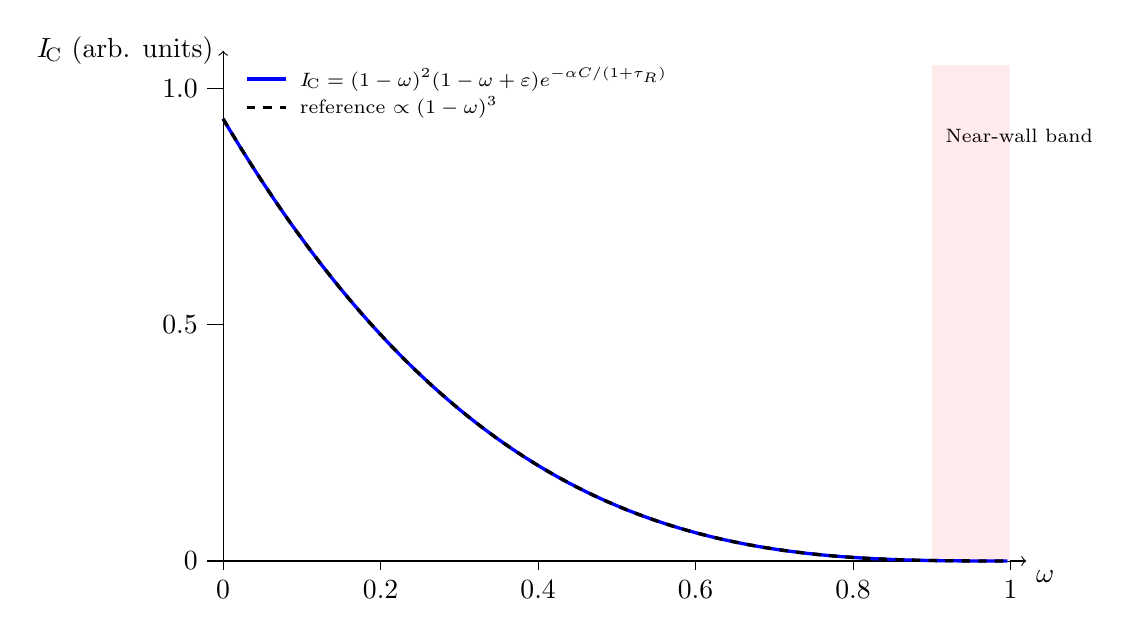
\begin{tikzpicture}[x=10cm,y=6cm]
    % axes box
    \draw[->] (0,0) -- (1.02,0) node[below right] {$\omega$};
    \draw[->] (0,0) -- (0,1.08) node[left] {$I_{\!\mathrm{C}}$ (arb. units)};
    % ticks (x)
    \foreach \x/\lbl in {0/0,0.2/0.2,0.4/0.4,0.6/0.6,0.8/0.8,1/1} {
      \draw (\x,0) -- ++(0,-0.02) node[below] {\lbl};
    }
    % ticks (y)
    \foreach \y/\ylbl in {0/0,0.5/0.5,1/1.0} {
      \draw (0,\y) -- ++(-0.02,0) node[left] {\ylbl};
    }
    % near-wall shaded band: ω in [0.90, 0.999]
    \fill[red!8] (0.90,0) rectangle (0.999,1.05);
    \node[anchor=west] at (0.905,0.90) {\scriptsize Near-wall band};

    % constants for curves (numerically inlined)
    % Kconst = exp(-alpha*C/(1+tauR)) with alpha=1, C=0.20, tauR=2.0 => exp(-0.2/3) ≈ 0.9355
    % epsilon = 1e-8 ~ 0.00000001

    % solid curve: IC = (1-ω)^2 (1-ω+ε) * Kconst
    \draw[very thick,blue,domain=0:0.999,samples=220,smooth,variable=\w]
      plot ({\w},{ (1-\w)*(1-\w) * (1-\w+0.00000001) * exp(-0.2/3.0) });

    % dashed reference: proportional to (1-ω)^3 (same constant factor)
    \draw[very thick,dashed,domain=0:0.999,samples=220,smooth,variable=\w]
      plot ({\w},{ (1-\w)*(1-\w)*(1-\w) * exp(-0.2/3.0) });

    % simple legend
    \draw[very thick,blue]   (0.03,1.02) -- (0.08,1.02);
    \node[anchor=west]       at (0.085,1.02) {\scriptsize $I_{\!\mathrm{C}}=(1-\omega)^2(1-\omega+\varepsilon)e^{-\alpha C/(1+\tau_R)}$};
    \draw[very thick,dashed] (0.03,0.96) -- (0.08,0.96);
    \node[anchor=west]       at (0.085,0.96) {\scriptsize reference $\propto (1-\omega)^3$};
  \end{tikzpicture}

  \caption{Near-wall cubic integrity fall. Solid curve uses $F=1-\omega$ and $S=-\ln(1-\omega+\varepsilon)$ in the composite identity; dashed is $(1-\omega)^3$ scaled by the same constant.
  \textbf{Parameters}: $(C,\tau_{R})=(0.20,\,2.0)$, $\alpha=1$, $\varepsilon=10^{-8}$.
  \textbf{Contract}: $(a,b,\varepsilon,p,\alpha)=(-3.7280384,\,10.856631,\,10^{-8},\,3,\,1.0)$.
  \textbf{Face policy}: \texttt{post\_clip+guard}.
  \textbf{Budget}: not applicable (derived curve).}
  \label{fig:near-wall-cubic}
\end{figure}
